\setchapterpreamble[u]{\margintoc}
\chapter{介绍}
\labch{介绍}

\section{灵感}

许多现代教科书都采用一种显眼的旁白排版,在旁白中可以展示图片,表格,标记等一切可以展示的东西。有证据表明,这种排版通过分离主体文本和辅助文本,有助于作者组织论述。同时,这些引用的辅助文本离主体文本非常近,方便读者查阅。

本文档并不是为了论证这种 1.5 栏宽边排版的好坏,因为已经有许多人在做类似的事情了。本文档的目的在于让读者用好 kaobookCJKsc 模板,同时也会介绍该类型的特点。

kaobookCJKsc 主要灵感来自于这篇\href{https://3d.bk.tudelft.nl/ken/en/2016/04/17/a-1.5-column-layout-in-latex.html}{博客},并且命名来自于原作者的名字 Ken Arroyo Ohori 首字母的缩写——原作者慷慨的授权我基于他的论文样式来创作这份模板。因此,如果你想用这种宽边排版制作你的书籍,可以去读一读他的博文。

你可能已经注意到了,另一个灵感来源是 \href{https://github.com/Tufte-LaTeX/tufte-latex}{Tufte-Latex} 模板。设计的本质其实是相似的,因为事实上,已有的这些模板已经足够好了,很难去彻底的提升。但是,我的想法是希望这份模板能比 Tufte-Latex 更灵活。比如,我尝试只用标准的包,并尽量减少从零设计。\sidenote{这也意味着理解并贡献这份模板会变得很容易。确实,许多特性还有待改进,如果感兴趣,就来 Github 主页吧。}因此,对于一些包提供的特性,如果你读了相关的文档,自定义应该非常容易。

在这本书里,我会介绍这份模板的主要特性,并提供如何使用和修改相关特性的信息。让我们开始吧。

\section{是什么}
\labsec{does}

\Class{kaobookCJKsc} 模板更多关注文档结构,而不是文档样式。正如著名的 \LaTeX 原则强调的,结构和样式应该尽可能分开。这份模板将只提供命令、环境以及一些用于定制的接口。实际上,有些样式相关的设置已经内置在模板中了,但用户仍可以自由定制。

\noindent 主要特性如下:

\begin{description}
	\item[页面排版] 降低了正文宽度以提高可读性,并且让出空间给文本注释以展示更多元素。
	\item[章节标题] 与 Tufte-Latex 不同的是,提供了多种章节标题,可以在本文档查看示例。
	\item[页面标题] 平铺整个页面,并且包含了留白。在双页模式下,将交替显示章节名和小节名。\sidenote{这也是区别于 Tufte-Latex 的地方。}
	\item[印刷材料] 已重新定义命令 \Command{frontmatter},\Command{mainmatter} 和 \Command{backmatter},以便在主要内容中自动具有宽边距,在前面和后面的内容中具有窄边距。但是,页面样式可以随时更改,即使是在文档的中间。
	\item[文本注释] 我们提供命令 \Command{sidenote} 和 \Command{marginnote} 将文本放在页边距中。\sidenote[][-2mm]{sidenote 有编号(像这样!),而 marginnotes 没有编号}
	\item[注释图表] \Environment{marginfigure} 和 \Environment{margintable} 是两个很有用的环境,允许你在页边距中放置数字和表格。(参见\reffig{marginmonalisa}).
	\item[注释目录] 既然我们有很宽的页边距,为什么不在其中添加一个小目录呢?参考 \Command{margintoc}。
	\item[超链接] 默认加载 \Package{hyperref},我们尝试以合理的方式添加书签;特别是,书签级别会在 \Command{appendix} 和 \Command{backmatter} 中自动重置。此外,我们还提供了一个小的包来简化文本其他部分的引用。
	\item[参考文献] 我们希望读者能够知道引用了什么,而不必每次都走到文档的末尾,因此引用会出现在页边空白处以及末尾,就像在 Tufte Latex 中一样。然而,与该模板不同的是,您可以根据自己的意愿自由定制引文。
\end{description}

\begin{marginfigure}[-3.5cm]
	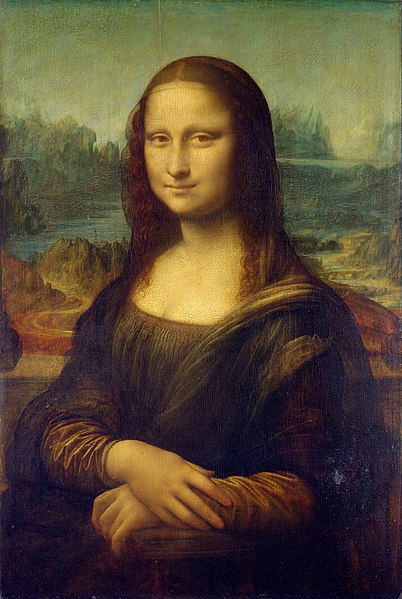
\includegraphics{monalisa}
	\caption[The Mona Lisa]{蒙娜丽莎\par\url{https://commons.wikimedia.org/wiki/File:Mona_Lisa,_by_Leonardo_da_Vinci,_from_C2RMF_retouched.jpg}}
	\labfig{marginmonalisa}
\end{marginfigure}

标题页、目录和前言的顺序可以很容易地更改,就像在任何 \LaTeX 文档中一样。此外,该模板基于 \KOMAScript 的 \Class{scrbook},因此它继承了原模板的所有优点。

\section{不是什么}
\labsec{doesnot}

正如预期的那样,该书的进一步定制将留给用户。可以肯定的是,每本书都有相似的旁注、页边数字等,但每本书都有自己独有的字体、目录风格、特殊环境等等。因此,除了类之外,我们只提供合理的默认值,但如果不需要这些特性,则可以忽略它们。这些特殊包位于样式目录中,其组织如下:

\begin{description}
	\item[kaoCJKsc.sty] 包含宏的最重要定义和页面排版规范。这是 \Class{kaobookCJKsc}	的核心。特殊功能包括:最常用的 \LaTeX 包已经自动加载;更改默认排版有一定的灵活性;一些特殊的环境(周围有彩色框、浮动或带计数的组件)是预定义的。\sidenote{参见\refch{引用}。}这是模仿 \Package{biblatex} 的。
	\item[kaorefsCJKsc.sty] 包含一些有用的命令来管理标签和引用,再次确保始终以一致的方式引用相同的元素。
	\item[kaotheoremsCJKsc.sty] 对于数学环境的样式,可以选择将其包装在彩色的 \Package{mdframed} 块中,如本文档所示,也可以不包装。
	\item[kaoWinCJKsc.sty] 提供 Windows 平台相关的设置。
	\item[config.tex] 存放一些无法放入样式文件的配置。
\end{description}

\marginnote[2mm]{大胆的用户可能会想编辑其中一些软件包。如果他们能给我寄来他们所能做到的例子,我将非常高兴!}

在本书的其余部分中,我将假设读者不是使用 \LaTeX 的新手,并参考本课程中使用的软件包的文档,了解其中已经解释的内容。此外,如果读者不喜欢默认设置,我假设读者愿意对提供的样式、环境和命令包进行少量编辑。

\section{如何用}
\labsec{howtouse}

先从 GitHub 仓库:\url{https://www.github.com/xuehao/kaobookCJKsc} 下载模板。

模板的使用方式有很多种。第一种是基于本文档项目,找到 main.tex 文件编辑即可;根据自己的需要删除部分文本,复制粘贴,重新创作。也可以基于另外两个 minimal 项目进行创作,他们是一个简化版本。无论如何,本文档项目都是最好的示例,你可以发现一些有用的特性,加入你自己的项目中。

对于想重头创建项目文档的用户,可以按照如下示例,先创建项目结构。默认使用时,文档结构如下所示\marginnote{译者注:注意 styles 文件夹不可以重命名,否则需要修改所有模板中的路径。}:

\begin{lstlisting}[style=kaolstplain]
	.
	├── styles
	│   ├── kaobiblioCJKsc.sty
	│   ├── kaobookCJKsc.cls
	│   ├── kaoCJKsc.sty
	│   ├── kaoWinCJKsc.sty
	│   ├── kaohandtCJKsc.cls
	│   ├── kaorefsCJKsc.sty
	│   ├── kaotheoremsCJKsc.sty
	│   └── config.tex
	├── main.tex                # 你的 LaTeX 文件
	├── Compiling.cmd
	└── Cleaning.cmd
\end{lstlisting}

编译同样需要使用命令行工具,切换到项目目录依次使用以下命令执行编译过程\marginnote[]{译者注:为了方便,译者提供了编辑好的编译脚本 \textbf{Compiling.cmd}。搭配 MiKTeX 发行版,已经在 Windows 10 平台上稳定使用。}:

\begin{lstlisting}[style=kaolstplain]
xelatex main                                  # 预编译模板
makeindex main.nlo -s nomencl.ist -o main.nls # 编译索引
makeindex main                                # 编译索引
biber main                                    # 编译参考文献
makeglossaries main                           # 编译字母表
xelatex main                                  # 再次编译模板
xelatex main                                  # 两到三次
xelatex main                                  # 防止边注错位
\end{lstlisting}

一般情况,按脚本顺序编译完即可,不会有错误。如有问题,可以去社区 \url{https://tex.stackexchange.org} 寻找答案,记得加上 kaobook 标签。当然,也可以在 GitHub 上创建 issues 或直接发邮件给我。

\section{\LaTeX 工作室}

众所周知,主流的 \LaTeX 发行版自带的编辑器非常难用。内置的编译流程也不太全面,无法做到一键编译。\marginnote{译者注:当然,搭配译者制作的一键编译工具,可以缓解一些不便之处!}为了实现高效编辑、简单编译、快速预览,这里推荐一套开源免费又轻巧好用的 \LaTeX 编译套装。推荐的方案是 \href{https://miktex.org/}{MiKTeX} 发行版,\href{https://code.visualstudio.com/}{Visual Studio Code} 编辑器搭配 \href{https://marketplace.visualstudio.com/items?itemName=James-Yu.latex-workshop}{\LaTeX\ Workshop} 插件。\marginnote{译者注:方案选择的首要原则是稳定,其次是跨平台,最后是免费。}

搭建自己的编译套装的前提是,\textbf{你必须了解你的编译工作流!}也就是说,针对你的文档项目,必须能使用前一小节介绍的命令行方式把完整的编译过程成功跑一遍。如果没有的话,大概率可以说明,你对 \LaTeX 编译工作流并不理解,后续对 Visual Studio Code 的配置也不可能正确。

在 Windows 平台下,要实现命令行完整编译的流程,需要安装以下几个工具:

\begin{lstlisting}[style=kaolstplain]
	\item 一款支持命令行工具的 \LaTeX 发行版,TeX Live 或 MiKTeX 等。
 	\item 默认支持的字体
 	\item 用于生成字母表的 Perl 工具
\end{lstlisting}

译者推荐安装 \href{https://miktex.org/}{MiKTeX} 发行版,选择 MiKTeX 有两个原因,其一是安装包很小,便于安装;其二是占用空间少,缺失的包会自动下载。Windows 平台安装完成后,打开命令提示符 CMD 输入以下命令测试(参见\reffig{marginmiktex}):

\begin{lstlisting}[style=kaolstplain]
	> xelatex --version
	MiKTeX-XeTeX 4.8 (MiKTeX 22.3)
	...
\end{lstlisting}

\begin{marginfigure}
	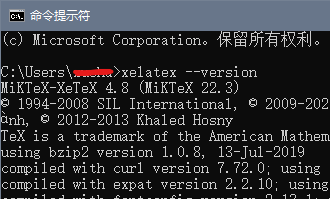
\includegraphics{miktex}
	\caption[MiKTeX]{MiKTeX}
	\labfig{marginmiktex}
\end{marginfigure}

简体中文模板默认使用美观、大方又开源的 \href{https://github.com/googlefonts/noto-cjk}{Google Noto} 字体。另外,原版英文字体需安装 liberation 系列字体,一并安装。\marginnote{译者注:字体备份 \url{https://pan.baidu.com/s/1r7qphMtlCdT9M3q26cokfA?pwd=uc75}}

除了字体,创建字母表页依赖 Perl 工具。为了后期的顺利编译,我们还需要安装 Perl,这里推荐安装 \href{https://strawberryperl.com/}{Strawberry Perl}。如果不需要字母表功能,可以不用安装,删除相关代码即可。

至此,已经可以愉快的使用命令行工具生成完整文档了。如上所述,我们继续安装 Visual Studio Code 以及其 \LaTeX Workshop 插件,以便实现高效编辑、自动编译、快捷预览等功能。

如果你之前使用命令行工具成功编译过你的项目,那么你一定会发现项目目录中多了很多杂七杂八的文件。每次删除都非常麻烦,一不小心还会删除自己的文件。\marginnote{译者注:对习惯命令行编译的用户,译者也慷慨地提供了一键清理工具 \textbf{Cleaning.cmd}。这也未尝不是一个好办法。}\LaTeX 项目需要多次编译,每次编译会依赖前一次生成的信息。对于我们这个工作流,编辑器插件虽然提供了自动清除功能,但由于其调用时机不确定,经常影响编译结果,所以不建议大家使用。因此,除非项目编译失败,编译过程中切记不要删除这些中间文件!只有确保文档创建成功后,再一次性清理。
